\section{Result}
\label{sec:result}

Figure~\ref{fig:eurusd-tick-analysis} presents an exploratory data analysis of EUR/USD tick data for January 2026. The top panel shows that the mid-price evolves broadly continuously but with intermittent jumps, while the bid-ask spread is highly concentrated at the minimum tick size with an extended right tail characteristic of illiquid periods. The middle panel reveals strong intraday seasonality in the spread, with compression during the overlapping London--New York session and widening during the Asian session and around macroeconomic announcements; the distribution of one-minute log returns exhibits the heavy tails and excess kurtosis typical of high-frequency data. The bottom panel confirms that trading intensity peaks at market open and at the US open, and that annualised daily realised volatility fluctuates substantially across the month---evidence of the time-varying dependence structure that the HMM framework is designed to capture.

\begin{figure}[h!]
    \centering
    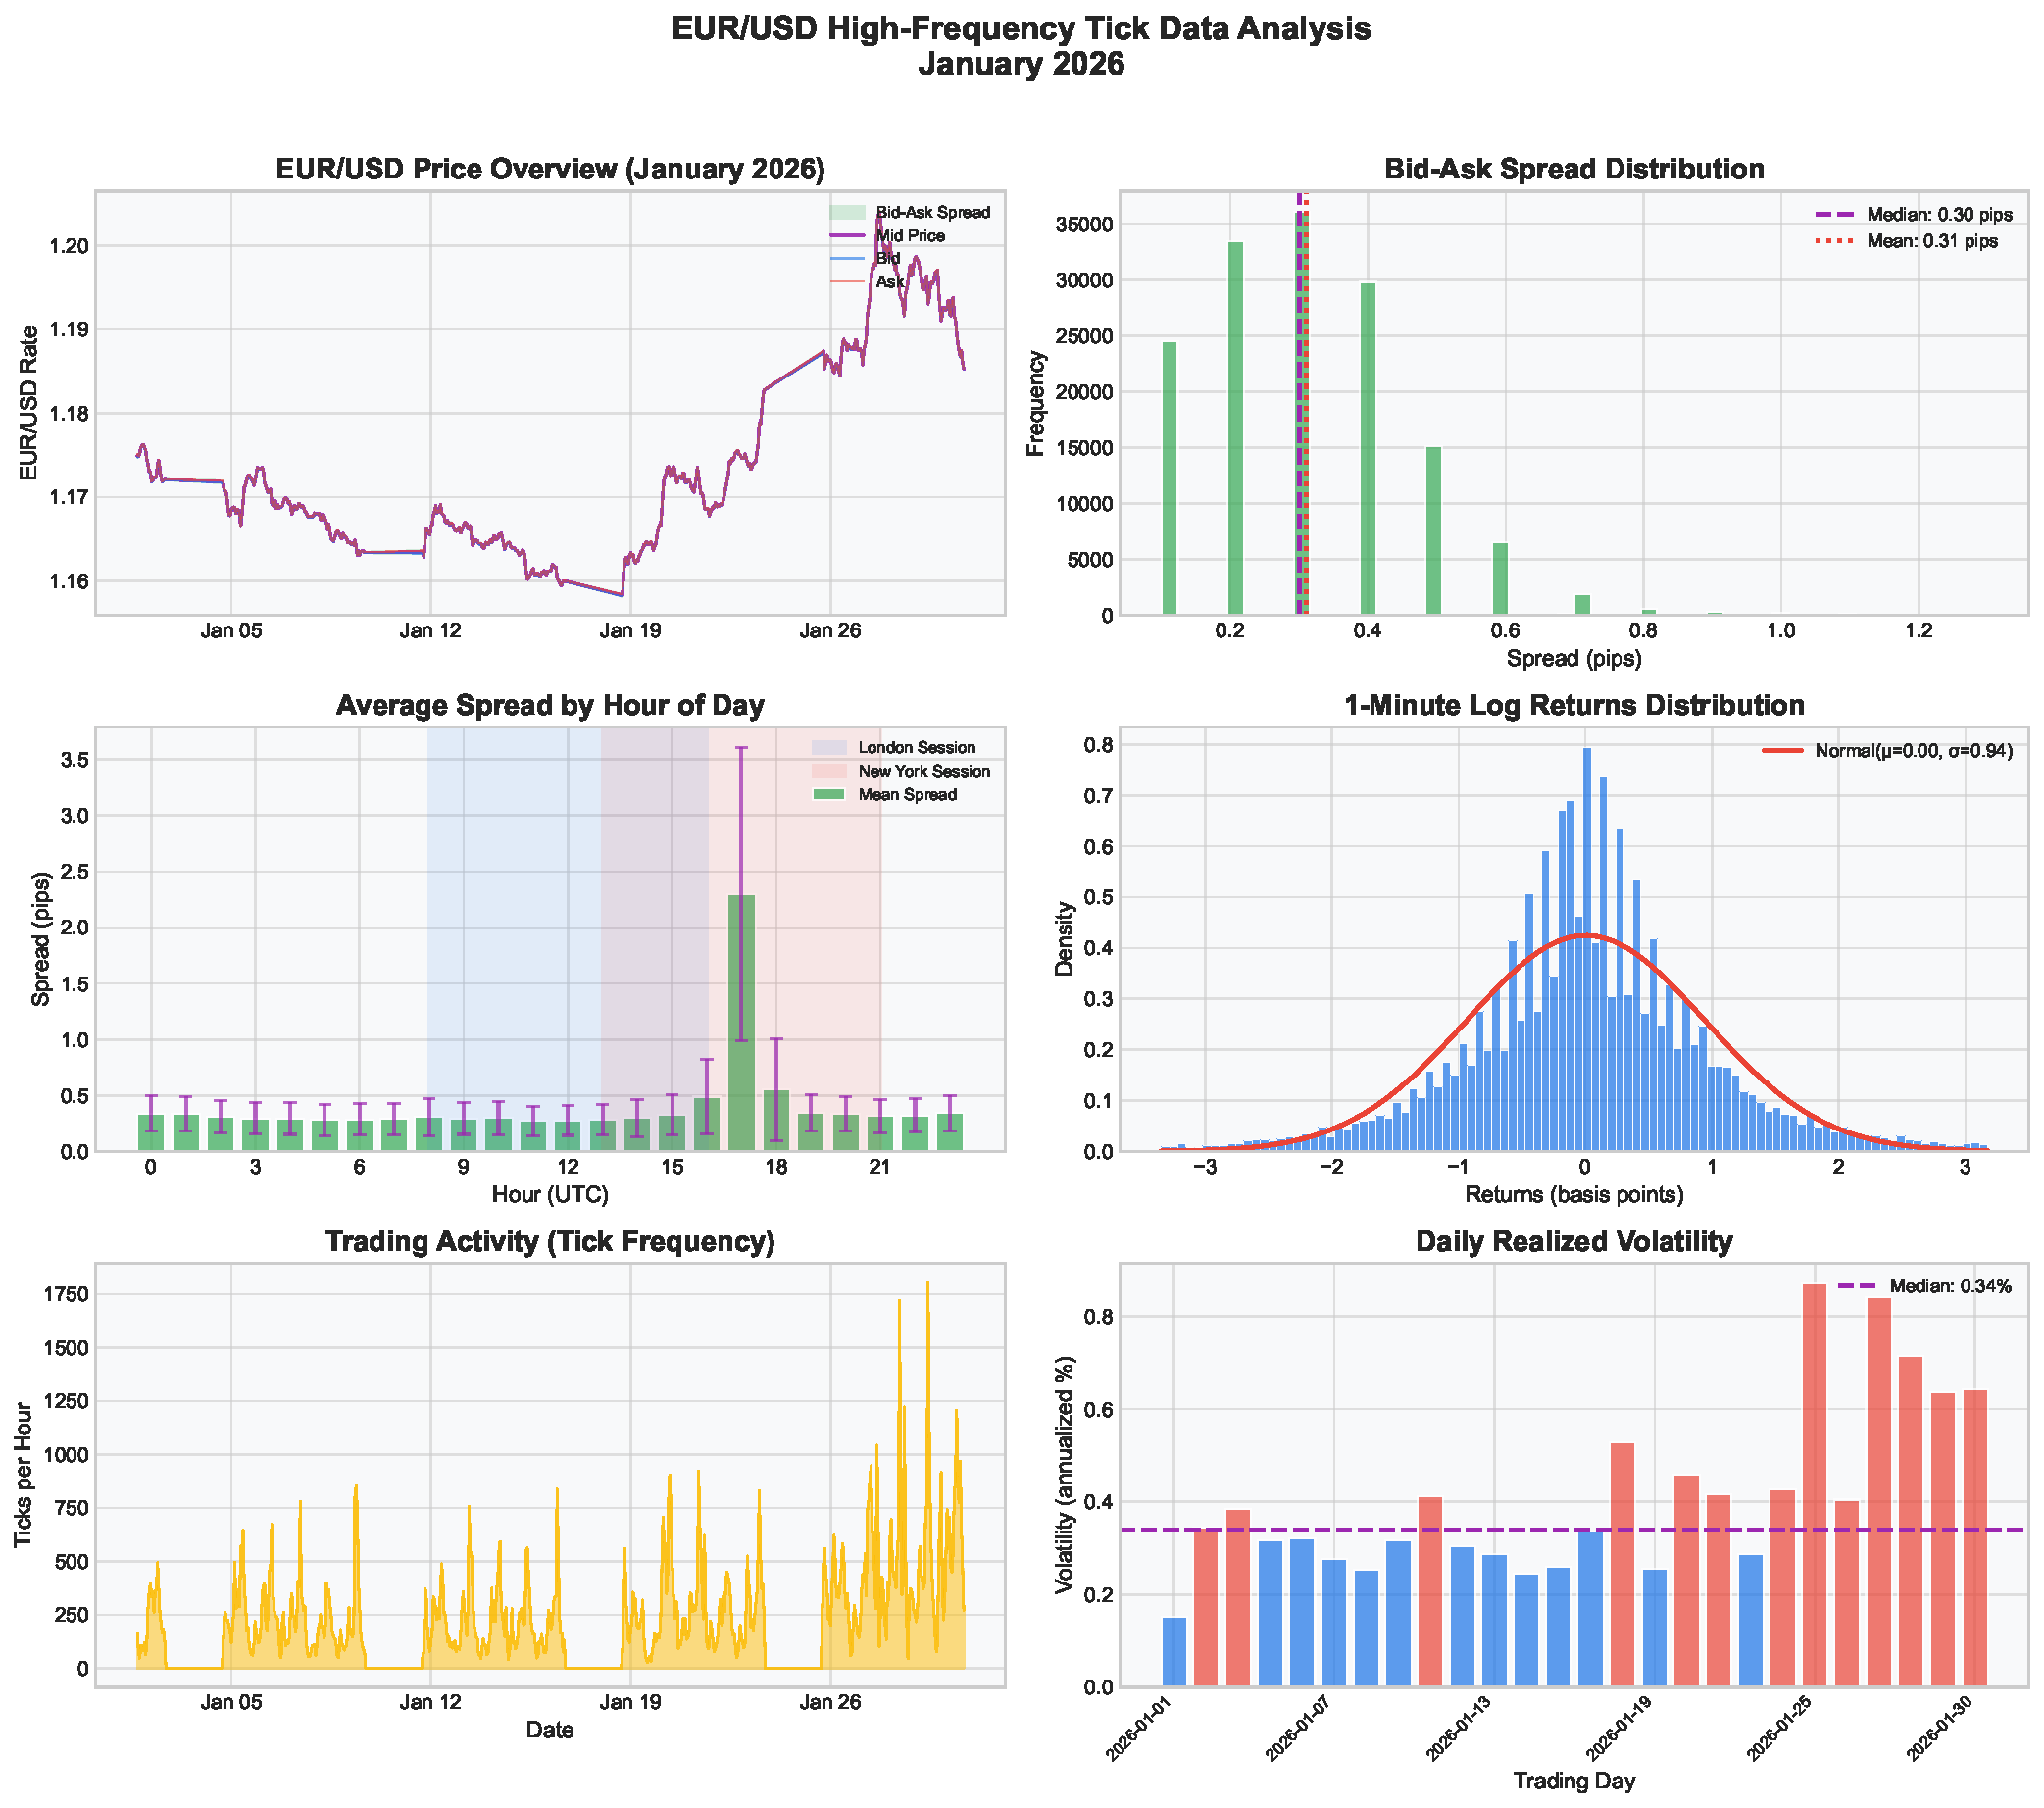
\includegraphics[width=0.6\linewidth]{plots/eurusd_tick_analysis.pdf}
    \caption{Exploratory data analysis of EUR/USD tick data for January 2026. The panels display the price evolution and bid-ask spread distribution (top); intraday spread seasonality highlighting the London and New York sessions, alongside the leptokurtic distribution of 1-minute log returns compared to a Gaussian benchmark (middle); and hourly trading activity frequency alongside annualized daily realized volatility (bottom).}
    \label{fig:eurusd-tick-analysis}
\end{figure}